%!TEX root = ../main.tex
\section{Modelling a DC motor}
This section deals with the modelling and parameterisation of a brushed DC motor, specifically the Pittmann 9234 24V servomotor.
Figure \ref{fig:dcmotormodel} is a simple model of a DC motor.
The parameters of this model will be estimated by experimentation.

\begin{figure}[!h]
	\centering
	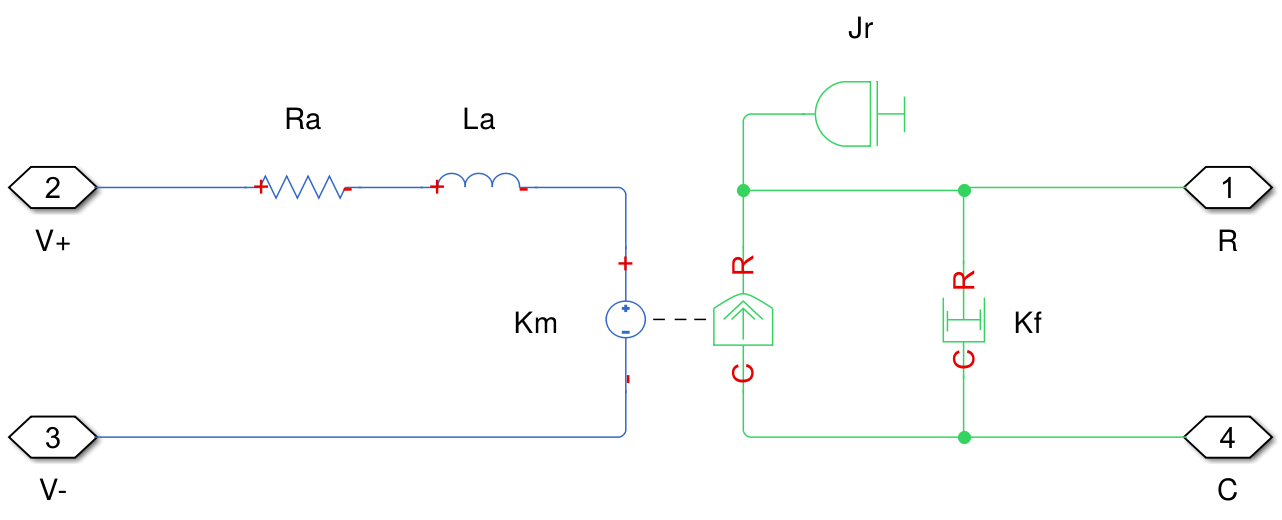
\includegraphics[width=\linewidth]{graphics/dcmotormodel.png}
	\caption{Simulink model of a brushed DC motor.}
	\label{fig:dcmotormodel}
\end{figure}

For the experiments a test setup is supplied. 
A diagram of the setup can be seen in figure \ref{fig:motorsetup}. 
As can be seen, two motors are connected by the shafts through an external inertia.
The shafts of the two motors will rotate in opposite directions given the same voltage.
To simulate this, a gearbox (called Inverter on the figure) with gear ratio -1:1 is placed between the two motors.
Finally, the Pittmann 9234S007-R1 is equipped with an encoder to allow for monitoring of the angular velocity of the shaft.


\begin{figure}[!h]
	\centering
	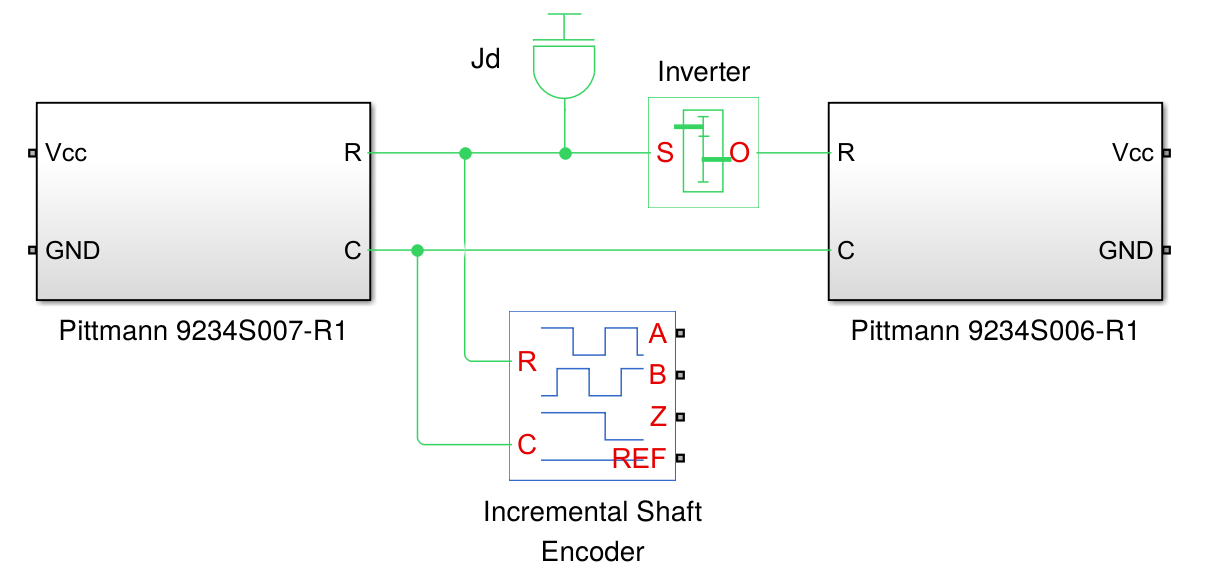
\includegraphics[width=.8\linewidth]{graphics/motorsetup.png}
	\caption{Simulink model of the motor setup provided for the project.}
	\label{fig:motorsetup}
\end{figure}

\subsection{Voltage Constant - $K_e$}
\label{sec:voltconstat}
The voltage constant describes the relationship between applied voltage and the resulting angular velocity of the rotor:
\begin{equation}
	\label{eq:voltconstant}
	K_e\omega_r = V_{cc}
\end{equation}
where $\omega_r$ is the angular velocity of the rotor and $V_{cc}$ is the voltage across the motor.
From equation \ref{eq:voltconstant} it is apparent that $K_e$ can be determined if the voltage across the terminals of the motor is measured while the motor is being run at a known velocity.
The experiment is conducted as follows:
A voltage is applied across the terminals of the Pittmann 9234S006.
The resulting velocity of the assembly is monitored using the encoder on the Pittmann 9234S007.
Across the terminals of this motor is now only the back-EMF.
This value is recorded.
Figure \ref{fig:velvsvolt} shows the recorded data. 
As is expected, there is a highly linear relationship between the voltage and velocity.
The final value of $K_e$ is determined by averaging and then dividing the collected data.
$$K_e=\frac{V_{cc}}{\omega_r}=0.0360$$
This value is within 1.2\% of the value given in the datasheet \cite{pittmann}.

\begin{figure}[!h]
	\centering
	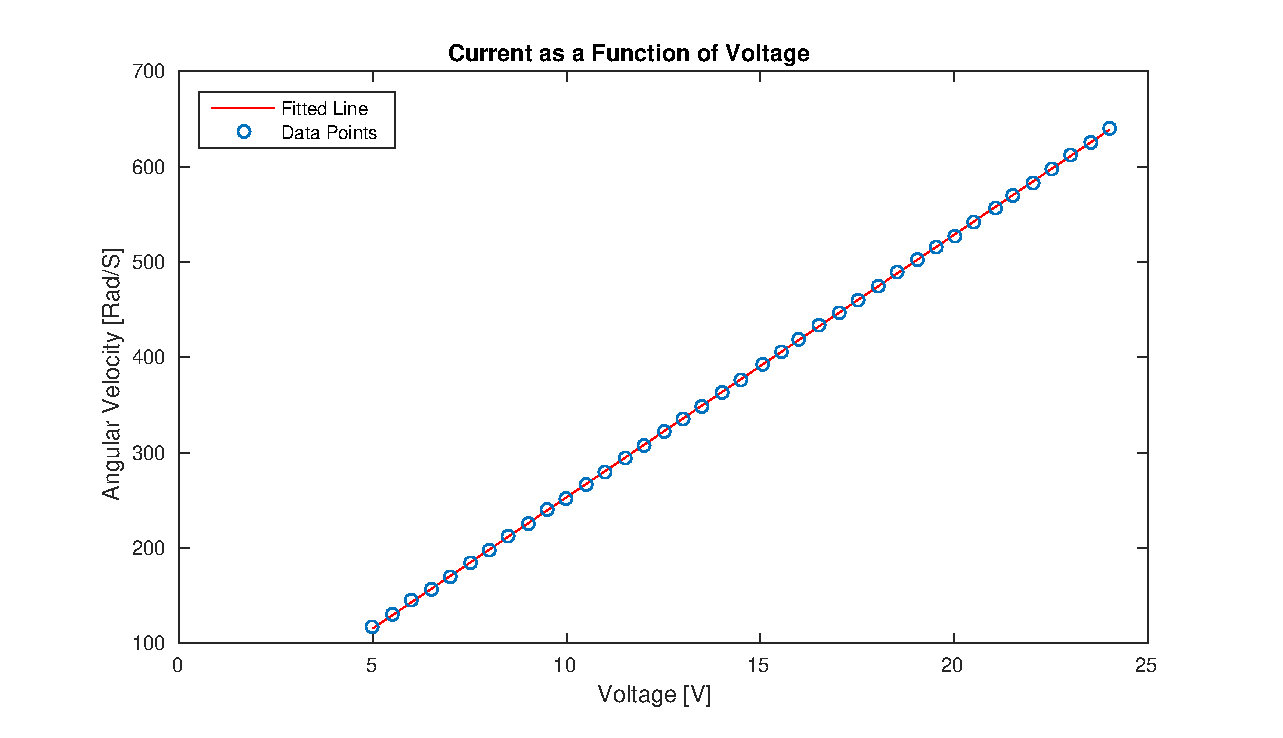
\includegraphics[width=\linewidth]{graphics/vvsrpm}
	\caption{Angular velocity of the shaft at different voltages.}
	\label{fig:velvsvolt}
\end{figure}

\subsection{Armature Resistance - $R_a$}
\paragraph{Method I}~\\
The armature resistance, $R_a$ in figure \ref{fig:dcmotormodel}, can be found simply by applying Ohm's law.
The current through a resistor is well defined when a voltage is applied across it.

\begin{figure}[!h]
	\centering
	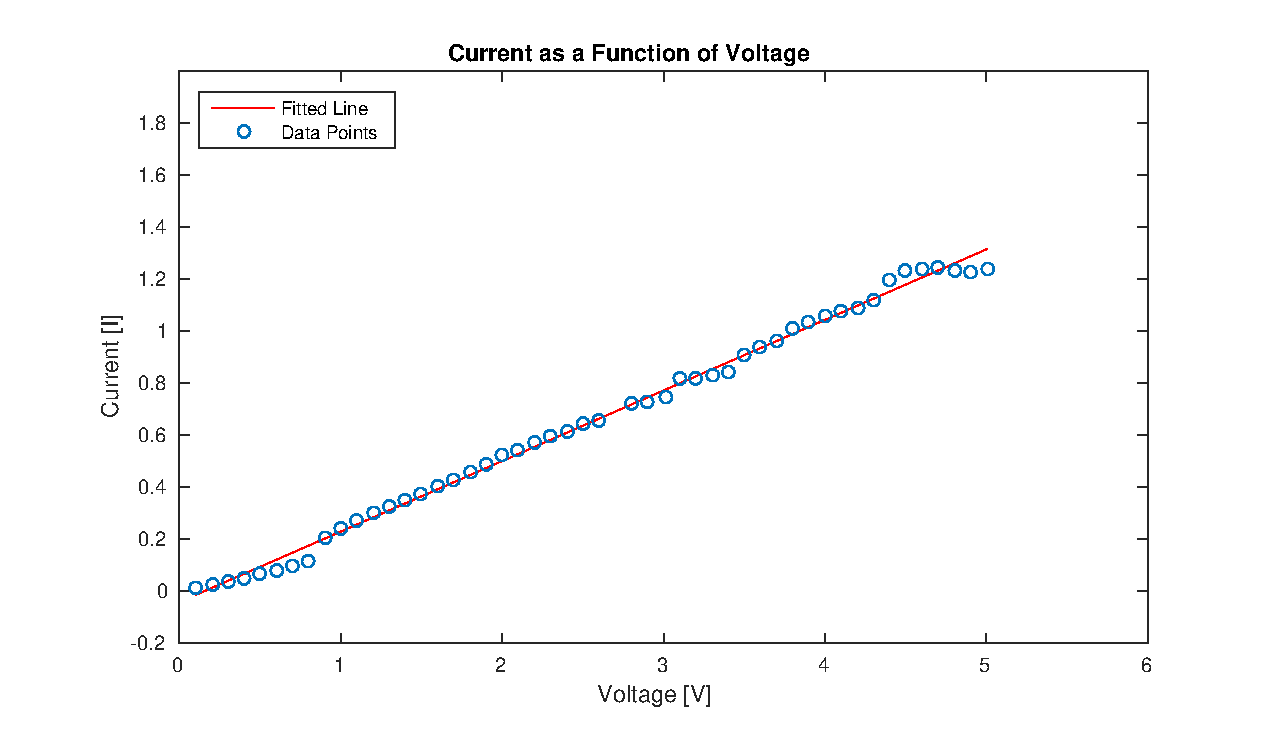
\includegraphics[width=\linewidth]{graphics/raplot}
	\caption{Current as a function of voltage with the rotor blocked.}
	\label{fig:raplot}
\end{figure}

However, when the rotor is spinning, the circuit produces back-EMF.
This counters the input voltage, effectively lowering the current through $R_a$.
In order to avoid this effect the rotor is blocked.
Since, with a blocked rotor, there will be no change in voltage in the system, the inductor acts as a short circuit, reducing the circuit to a voltage across a resistor. 

Figure \ref{fig:raplot} shows the data collected in order to determine the value of the armature resistance.
A voltage is applied across the terminals at 0.5 V.
According to the datasheet \cite{pittmann} the current at maximum allowed continuous torque is 1.75 A.
This current is reached at 5 V, therefore, the measurements stop there.
As can be seen from the figure, a line is fitted to the data.
This is done using the linear least squares method with the following result:
$$I(V)=0.272\cdot V-0.042$$
with $R^2=0.995$.
Since for the plot $I(V)$:
$$R_a = \frac{1}{\text{slope}} = 3.683\Omega$$
This value is significantly higher, approximately 25\% higher, than the value given in the datasheet.
Additionally, the final data points seem to become irregular.
This is likely caused by the high currents drawn by the motor at these voltages warming the motor and therefore slightly altering the characteristics of the resistor.

For these reasons it has been decided to pursue a different means of determining the armature resistance:
\paragraph{Method II}~\\
This method makes use of the voltage constant found in section \ref{sec:voltconstat}.
By expanding $V_{cc}$ in equation \ref{eq:voltconstant} an expression for $R_a$ can be found:
\begin{equation}
	\label{eq:voltconstantexpanded}
	K_e\omega_r = V_{cc} = I_aR_a\quad \Rightarrow \quad R_a = \frac{\omega_rK_e}{I_a}
\end{equation}
Similarly to the experiment in section \ref{sec:voltconstat}, one motor is used to spin the other to speed.
This time, however, the terminals of the Pittmann 9234S007 are connected through a power resistor, $R_e$.
Obviously then:

\begin{eqnarray}
	R_t =& R_a + R_e\\
	R_a =& \frac{\omega_rK_e}{I_a}-R_e
\end{eqnarray}

where $R_t$ is the total resistance in the system.
As the voltage across the terminals of the Pittmann 9234S006 is increased the resulting velocity and current is noted.
Finally, the armature resistance is found to be:
$$R_a = 3.715\Omega$$

This value, curiously, coincides with the one found using method I.
